\chapter{Workshop introduction} 

\begin{quote}
	Wildland fire science literacy is the capacity for wildland fire professionals to understand and communicate three aspects of wildland fire: (1) the fundamentals of fuels and fire behaviour, (2) the concept of fire as an ecological regime, and (3) multiple human dimensions of wildland fire and the socio-ecological elements of fire regimes \citep[][ Fig.~\ref{fig:WalletCard}]{mcgranahan2018}.
\end{quote}  

\begin{figure*}[!b] 

	\begin{center}
		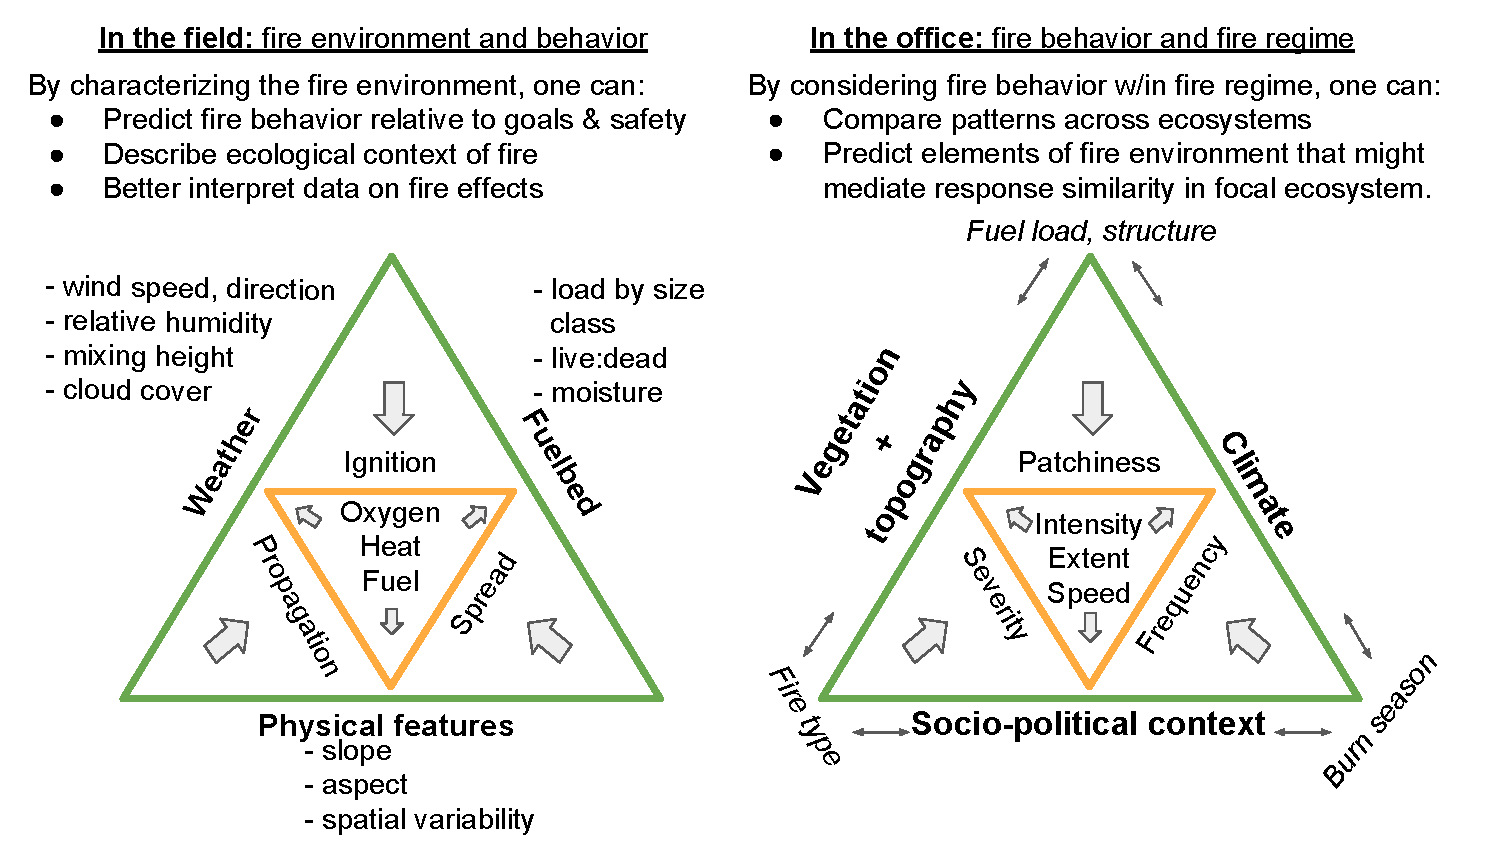
\includegraphics[width=1\textwidth]{WalletCard}
		\ImageCredit{\citet{mcgranahan2018}}
	\end{center}
	\caption{Two arenas of wildland fire science\textemdash the field and the office. 
	This figure helps fire professionals from each arena identify characteristics of the fire environment or fire regime that dominate their colleagues' perspective.  
	\label{fig:WalletCard} }  %(Fig.~\ref{fig:WalletCard})
\end{figure*}


\section{Known knowns} 

\section{Known unknowns}

\section{Unknown unknowns} 

